\documentclass[12pt,a4paper,notitlepage]{article}

\usepackage{./styles/plog1}

\addbibresource{plog1.bib}

\newcommand*{\foottitle}{Pente 3 - PLOG 2018}
\newcommand*{\boardsize}[1]{$#1$\texttt{x}$#1$}


\title{
	\vspace{-2\baselineskip}
	
\includegraphics[scale=0.15]{feuplogo.jpg}\\
	{\Huge Pente}\\
	{\Large \texttt{Prolog} Implementation of a Board Game}\\
	{\normalsize PLOG 2018}
}

\author{
	Bruno Dias da Costa Carvalho\hspace*{1.5em}\text{up201606517}
	\and
	Amadeu Prazeres Pereira\hspace*{1.5em}\text{up201605646} 
}

\begin{document}
\maketitle
\thispagestyle{empty}
\vspace*{-2\baselineskip}
\tableofcontents

\section{Introduction}
\label{sec:introduction}

This project's objective is to implement a board game using Prolog, with 3 different modes: Player vs Player, Player vs Bot and Bot vs Bot, with the Bot having 2 different difficulties. Our game is Pente.

We implemented all of Pente's rules (see below) and created proper abstractions and compound terms to represent boards, game states, and other repetitive data elements.
This will all be discussed below.

\section{Overview and History}
\label{sec:overview}

\textbf{Pente} is an \textit{abstract strategy board game}, played usually by two players, in which the aim is to create an unbroken chain of five stones \emph{or} to capture ten of the enemy's stones.

It was created in 1977 by Gary Gabrel at the restaurant \textsl{Hideaway Pizza}, in Stillwater, Oklahoma, USA.\supercite{pente-wikipedia}
Customers waiting for their orders to arrive would play a variation of the game on checkerboard tablecloths.\supercite{pente-wikipedia}

Some variations allow for more than two independent players, and even teams, to play simultaneously. These require relaxing the winning conditions of the game to accommodate for the increased opposition --- namely requiring only a four-in-a-row for three or four players, and allowing mixed captures for teams.\supercite{pente-winning-moves}

\begin{wrapfigure}[12]{l}[2em]{0.33\textwidth}
	\vspace*{-1\baselineskip}
	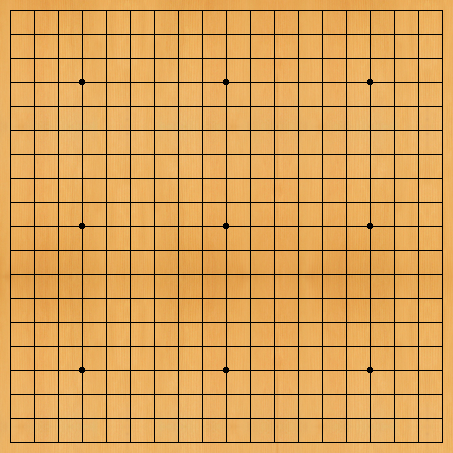
\includegraphics[scale=0.4]{goban.png}
	\caption{\boardsize{19} \textit{Go} board. \label{fig:goban}}
\end{wrapfigure}

The game has many variations for two player games -- all of which have a common ancestry in \textit{Gomoku}, which has a significantly simpler rule-set.
All variations of the game are played in the style of \textit{Go}, on the intersections of a traditional \boardsize{19} \emph{Go} board with black and white pieces called \emph{stones}. One player, \textsl{White}, uses the white stones, and the other, \textsl{Black}, uses the black stones. Once placed on the board, stones may not be moved, but may be removed from the board if \emph{captured}.

Introductory or speed games may be played on the smaller \boardsize{9} or \boardsize{13} boards, but the tighter space makes it very difficult to generate common patterns of play.

\section{Game Rules}
\label{sec:rules}

The game's precise rules vary considerably throughout variations and sources. As such, we'll first review the common base rules and then discuss a few variations.

\subsection{Base rules}
\label{subsec:baserules}

Let's recall there are two winning conditions, same for White and Black:

\begin{itemize}
	\large
	\item Form an unbroken chain of 5 or more consecutive friendly stones --- vertically, horizontally or diagonally.
	\item Capture a total of 10 enemy stones.
\end{itemize}

\begin{wrapfigure}[8]{r}[2em]{0.3\textwidth}
	\vspace*{-3\baselineskip}
	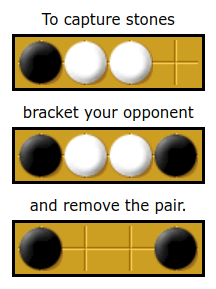
\includegraphics[scale=0.6]{capture.png}
	\caption{Capturing\supercite{pente-net} \label{fig:capture}}
\end{wrapfigure}

Unlike traditional \textit{Gomoku}, the chain may indeed have more than five consecutive stones.

\subsubsection{Captures}
\label{subsubsec:captures}

Captures occur when two friendly adjacent stones (and only two) become bracketed by a pair of enemy stones, in a configuration depicted in \autoref{fig:capture}. Captures may arise in any direction.

\subsection{Variations}
\label{subsec:variations}

Some sources add the following secondary rules.

\begin{itemize}
	\item White always plays first, in the center.\supercite{pente-renjunu, pente-wikipedia} This is unlike \textit{Renju} and \textit{Gomoku}.
	\item \textsl{Suicides} are not possible -- if a player places two adjacent friendly stones into a bracketed position --- for example, if White forms the second panel of \autoref{fig:capture} --- his stones are not captured.\supercite{pente-renjunu,pente-org,pente-wikipedia,pente-winning-moves}
	\item Tournament Rule: The first player's second move is restricted -- it must be at least three intersections away from the center (that is, outside the board's middle \boardsize{5}).\supercite{pente-net,pente-org,pente-wikipedia,pente-winning-moves}
\end{itemize}

We'll be using these three rules hereafter.

Other sources do not specify starting player (or choose Black) and do not require the tournament rule, at least for casual play. 

Among variations we find: suicides allowed, called \textit{poofs} (\textit{Poof-Pente}); harsher Tournament Rule (\textit{G-Pente}, \textit{D-Pente}); 3-in-a-row captures (\textit{Keryo-Pente}), and others.\supercite{pente-org,pente-net}

\section{Internal Representation}
\label{sec:internal}

Representing the game's board is fairly simple.
Every position in the \boardsize{19} board is in one of three states:
white piece, black piece, or empty. We'll represent the board using
an \boardsize{S} matrix (list of lists), whose elements are \textbf{w},
\textbf{b} or \textbf{c}, for each state respectively.
This matrix will be called \vt{Board}.

Now, each player has captured a certain number of pieces (an integer) and only plays pieces of a certain color (white or black). We'll represent the captures as a pair [\vt{Wc},\vt{Bc}], with no similar general abstraction for \textit{players} (it wasn't needed).

The overall game state will be represented by a \textit{game/5} data compound:
\begin{center}
	\comp{game(Board, P, [Wc,Bc], Turn, Options)}
\end{center}
where P is w or b according to who will play next, Turn is an integer starting at 0 that counts moves, and lastly, Options is a list that represents the game's options (see \autoref{subsec:options}).

\subsection{Definitions, Compounds and Abstractions}
\label{subsec:abstractions}

There are two more data compounds: \vt{val/4}, which holds a board evaluation (see \autoref{subsec:boardscoring}) and \vt{node/6}, which is a node in the bot's evaluation tree (see \autoref{subsec:bot}).

Several list data structures are abstracted away either by library  or auxiliary predicates which act on them: \vt{Move} is merely a row column pair [$R$,$C$]; \vt{Range} is a list [$I$,$J$] representing an interval (which includes $I$ and $J$); \vt{Cap} is the pair of captures [Wc,Bc]; the three compounds are usually kept unexpanded in variables \vt{Game}, \vt{Val}, \vt{Node}, \vt{Tree}, etc.

\subsection{Board Display}
\label{sec:boarddisplay}

It's possible to flip the board (display only, not representation) when it is Black's turn to play, as if the two players were playing face-to-face on a physical Go board. Naturally we adjust the identification of rows and columns. By default this is turned off.

To draw the board with text (on the console) we used unicode box-drawing characters (range \texttt{u+2500}--\texttt{u+257f}). The white and black pieces become filled and empty unicode circles, respectively. This assumes a dark-themed console --- white consoles will have the colors swapped.
Below the board you can see the pieces captured and the turn number.

For examples see \autoref{fig:earlygame}, \autoref{fig:midgame} and \autoref{fig:lategame} below.

\begin{figure}[bhtp]
	\centering
	\begin{minipage}{0.35\textwidth}
	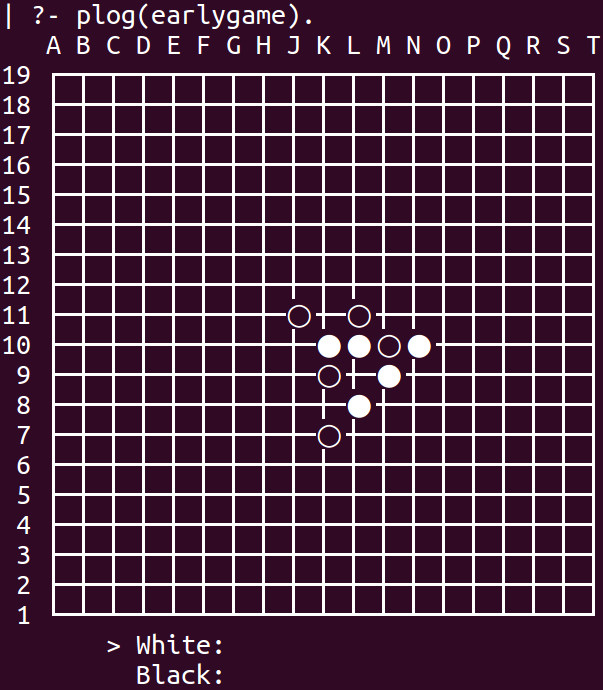
\includegraphics[width=\textwidth]{earlygame.png}
	\end{minipage}
	\begin{minipage}{0.45\textwidth}
		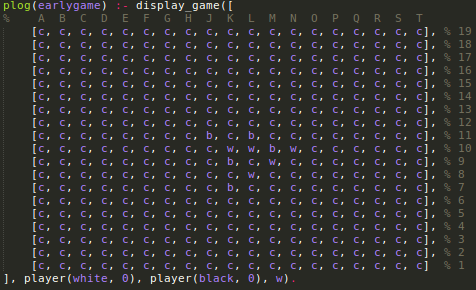
\includegraphics[width=\textwidth]{earlygame-code.png}
	\end{minipage}
	\caption{A game after 10 moves. It is White's turn to play.}
	\label{fig:earlygame}
\end{figure}
\vspace*{-2\baselineskip}
\begin{figure}
	\centering
	\begin{minipage}{0.35\textwidth}
		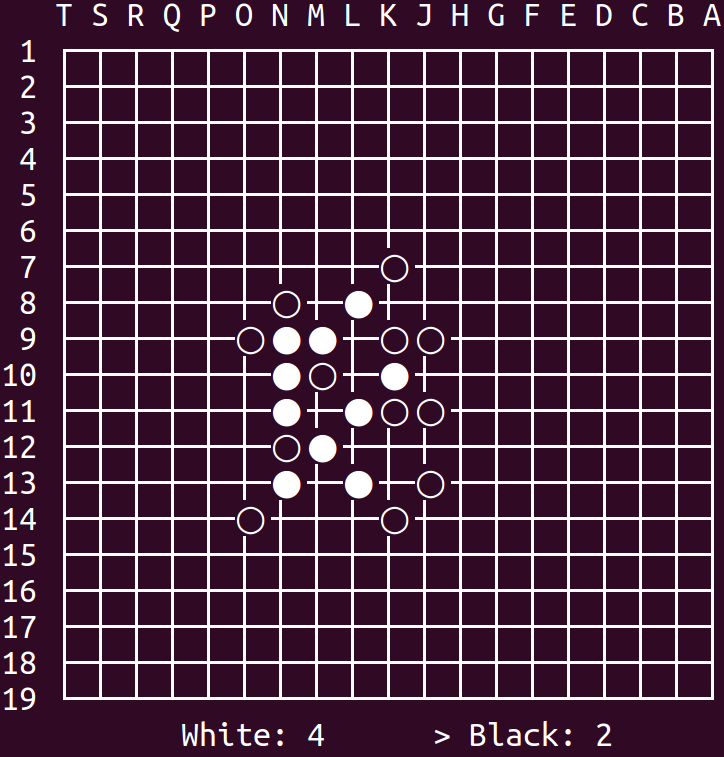
\includegraphics[width=\textwidth]{midgame.png}
	\end{minipage}
	\begin{minipage}{0.45\textwidth}
		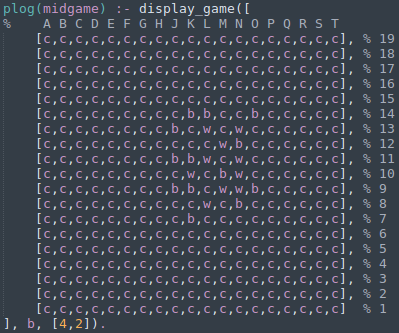
\includegraphics[width=\textwidth]{midgame-code.png}
	\end{minipage}
	\caption{A game after 29 moves. It is Black's turn to play.}
	\label{fig:midgame}
\end{figure}
\vspace*{-2\baselineskip}
\begin{figure}
	\centering
	\begin{minipage}{0.35\textwidth}
		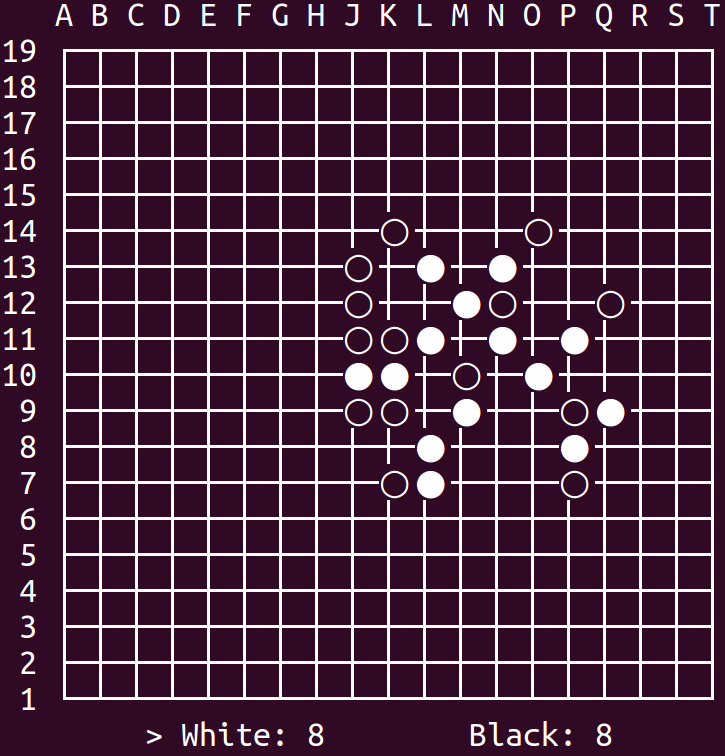
\includegraphics[width=\textwidth]{lategame.png}
	\end{minipage}
	\begin{minipage}{0.45\textwidth}
		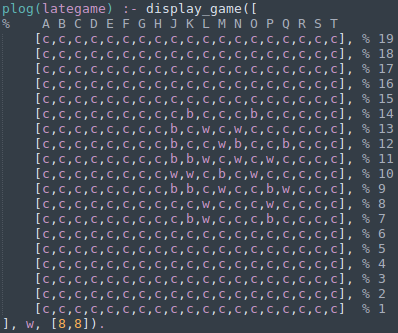
\includegraphics[width=\textwidth]{lategame-code.png}
	\end{minipage}
	\caption{A game after 44 moves. It is White's turn to play, and win at H11.}
	\label{fig:lategame}
\end{figure}

\section{Game Logic}
\label{sec:gamelogic}

The entry points are \vt{pente/[0,1]} and \vt{play/[0,1]}. The functors accept an \vt{OptionsList} argument specifying implementation details or game rules only; the game type --- Player vs Player, Player vs Bot and Bot vs Bot --- are chosen through a simple menu afterwards.

See also predicate \vt{help/[0,1]}.

\subsection{Options}
\label{subsec:options}

The options accepted in the \vt{OptionsList} argument of \vt{play/1} are the following (use \vt{help} or \vt{help(Option)} to get a description on the console):

\begin{itemize}
\item \vtb{board_size(S)} or \vtb{size(S)}, \vt{S} in $\{7,9,11,...\}$\\
Defines the board size (SxS), must be odd.
Default: 19.
\item \vtb{difficulty(D)}, \vt{D} in $\{1,2,3,4,5\}$\\
Sets the bot difficulty (with 5 being the most
difficult) by selecting a set of predefined values
for depth, padding and width. If given values for
depth, padding and width, these override those selected
by the difficulty.
\item \vtb{depth(D)}, \vt{D} in $\{0,1,2,3,...\}$\\
Depth of the bot's search tree.
\item \vtb{padding(P)}, \vt{P} in $\{1,2,3,...\}$\\
Padding of the active subboard used by the search tree.
\item \vtb{width([W1,W2,...])}, \vt{Wi} in $\{1,2,3,...\}$\\
For each search node on depth $i$ (top is depth 0)
recurse the search tree only for the $W_i$ best moves.
If the width is not defined for all the depths, the
last width in the list will be used repeatedly.
Please be mindful that bot runtime is $o(W1\times\cdots\times W_{D})$
on average per move.
\item \vtb{width(W)}, \vt{W} in $\{1,2,3,...\}$
Use the width W for all depths.
\item \vtb{flip_board(B)} or \vtb{flip(B)}, \vt{B} is \vt{true} or \vt{false}\\
Flip the board print on the console for Black's turn.
Default: false.
\item \vtb{tournament_rule(B)} or \vtb{rule(B)}, \vt{B} is \vt{true} or \vt{false}\\
Use the tournament rule.
Default: true.
\end{itemize}

\subsection{Valid Moves}
\label{subsec:validmoves}

In Pente, the player's possible moves do not depend on which player is going to play. The available moves are the same for each one.
With this in mind, we implemented several predicates that give us a list with all the possible moves a player can make: \vt{empty_positions/[2,3]}, \vt{valid_stones/[2-5]} and their \vt{within_boundary} counterparts.

\begin{itemize}[noitemsep]
\item \vtb{valid_moves/2}: \vt{valid_moves(+Board, -ListOfMoves)}\\
This gives the player all the empty positions on the board, does not take in consideration the game's turn or if the user wants to play using the tournament rule.
\item \vtb{valid_moves/3}: \vt{valid_moves(+Board, +Turn, -ListOfMoves)}\\
More specific than the previous one, it takes a Turn and makes sure that at the turn number 0 the only available move for the player is the center intersection, and at turn number 2 implements the Tournament Rule.
\item \vtb{valid_moves/4}: \vt{valid_moves(+Board, +Turn, +Rule, -ListOfMoves)}\\
Takes into account the game Turn and if the Tournament Rule is active or not.
\end{itemize}

\subsection{Validation and Execution of Moves}
\label{subsec:moves}

Input is expected quietly whenever it is the player's turn to make a move.
Moves are typed into the console like
\begin{center}
	\ttfamily K10.
\end{center}
and column K, row 10 is deduced. If invalid, new input will be silently expected.

When a player chooses a move it needs to be checked before being accepted. This is done by asserting the move is in the appropriate list of valid moves (see \vt{valid_move/[2-4]}) returned from one of the predicates described above.

Once the player move is valid we have to do several things:

\begin{enumerate}[noitemsep,label=(\roman*)]
	\item Place the player's stone at the given position.
	\item Check if that stone bracketed the opponent, in every one of the eight possible directions. In that case, remove those 2 stones from the board and add 2 captures to the player's total captures.
	\item Update the next player playing.
	\item Increment the game's turn by 1.
\end{enumerate}

Items (i) and (ii) above are carried out by \vt{place_stone/5} through the use of \vt{remove_dead_stones/5}. The whole process is \vt{move/3} as seen from the main game loop.

\subsection{Game Over}
\label{subsec:gameover}

In the end of every game iteration a test is performed by \textbf{game\_over/2} to check for either winning condition, for either player.

In case of victory, a message is displayed for that player and the game cycle is stopped, ending the game successfully. Otherwise the game must go on.

\subsection{Board Scoring}
\label{subsec:boardscoring}

Our board evaluation idea is simple in theory, but hard to implement \textit{effectively}. Consider an \boardsize{S} Board. It has $S$ rows, $S$ columns, $2S - 1$ diagonals parallel to the main diagonal -- we call them \textit{left} diagonals, as the longest starts on the top left -- and $2S - 1$ \textit{right diagonals}, perpendicular to the main diagonal. All of these are ways of splitting the two-dimensional Board into multiple one-dimensional \textsl{lists}.

Good Pente patterns might show up in any such list, namely four and five-in-a-rows, or simpler patterns at the beginning of the game. Hence we decided the value of a Board is determined entirely by the individual values of these lists. No two-dimensional patterns are recognized or searched for when evaluating a Board. The value of a game position is the board value plus a function of the player captures.

The Board's value is stored in compound \vt{val/4}:
\begin{center}
	\vt{val(RowValues, ColValues, LeftValues, RightValues)}
\end{center}

Board value is based entirely on \textit{list patterns}. Through \vt{pattern/2}, a \textsl{score} is given to each short pattern comprising one to six pieces all of the same color. From patterns as simple as\footnote{The dashes represent empty intersections}
\begin{center}
\tt	- W -
\end{center}
to patterns such as
\begin{center}
\tt	- W - W W - W W W - -
\end{center}
Scores range from $1$ for a single piece to $2^{100}$ for a five-in-a-row.

To score a given List, for every recorded pattern one counts its number of occurrences in List, multiples it by the pattern's score, and adds all of them up to get the value of List.

Patterns made with White pieces are positive (\vt{pattern/2}), those made with Black pieces are their negative. Scoring each list is done with \vt{evaluate/2}, which accumulates \vt{score/2}; the Board's total value is computed with \vt{evaluate_board/2}, and finally the value of the game position is computed with \vt{totalval/3}, which needs the player captures.

There are about $150$ patterns scored by hand, for a total of $300$ \vt{score/2} searches in every list\footnote{Predicates \vt{p/2}, \vt{e/1} and \vt{a/1} present different ways of investigating the score of a list}. Some of these are not very meaningful and can be removed to increase efficiency substantially, but we did two other things to speed up evaluation for the Bot:

\begin{itemize}
	\item Instead of evaluating an entire board every time with \vt{evaluate_board/2}, we use mostly \vt{reevaluate_board/4} which takes two Boards that differ by just one stone placement (one move), the initial Board's value, and computes the new Value, only having to reevaluate, most of the time, four new lists.
	\item Predicate \vt{evaluate/2} is dynamic and every new list evaluation result is stored using \vt{asserta} (the lemma idiom). This results in tens of thousands of clauses for \vt{evaluate/2} once the bot kicks in, making evaluation mostly a matter of lookup.
\end{itemize}

\subsubsection{Motivation}
\label{subsubsec:motivation}

If we create a decent, fast Bot but our hand-picked scores are very bad, they can be improved at a future time through machine-learning and self-play, or on a lower scale through simple experimentation.

By downscaling a two-dimensional board into multiple one-dimensional lists we lose tremendous amounts of information, but to look for various different two-dimensional patterns in a 19x19 board efficiently is just computationally infeasible. Look at Go for example.

Another idea we had was to look mostly/exclusively for forcing patterns on the board (possibly two-dimensional) like
\begin{center}
\tt - W - W W W - -
\end{center}
which require Black to respond locally, possibly twice; or even patterns like the \textit{tessera}
\begin{center}
\tt - W W W W -
\end{center}
which are win-in-one bar any captures. But these don't help the Bot play the first few moves in the game, are very hard-coded, are require much more knowledge of the game than the one we have.

\subsection{Computer Bot Moves}
\label{subsec:bot}

We made an elaborate, although static and largely imperfect Bot to play Pente which uses board evaluations for the lookahead tree.

The lookahead tree is \textit{not} (necessarily) binary. It's rooted in the current game position, its children are the possible moves being analyzed, and in general every subtree head is one move away from any of its children.
The tree is static: it has fixed depth and fixed width set at game startup, which do not change throughout (see \autoref{subsec:options}).

A node in the tree (and the tree itself) is represented by \vt{node/6}:
\begin{center}
\tt node(Board, P, Val, Cap, Children, Worth)
\end{center}
where P is the next player (the one making the move M that transforms the node into one of its children), Children is a key-valued ordered list of children nodes (empty list for leaves), and Worth is a score-like integer which is the current \textit{value} of the node.

The \textit{worth} of a node is initially just the value of the game position it is assigned, but it will change after the node has generated its children: once a subtree is generated, the worth of the leaf nodes bubbles up the tree naturally, according to the following rules:
\begin{itemize}
\item If a parent node generates a child node which is surely a losing position (for the child node's player), then the parent node is surely a winning position (for the parent node's player). Once this child node is found, no more child nodes need be generated any longer for this parent node. See \vt{build_children/3} and \vt{recurse_children}
\item The parent node is assigned the worth of the best of his children.\footnote{Remember White wants positive score/worth, Black wants negative score/worth} Before this, the children are ordered by worth. To ensure repeated bot games don't play out the same way, the children are clumped by worth, randomized within each clump, then put back together. See \vt{reorder_clumps/2}
\item If a parent node generates a child node which is surely a winning position (for the child node's player), then the parent node's player should not play the move leading to said child node position. This means the child node can be effectively discarded. See \vt{recurse_children_loop/5}. \footnote{Some care must be taken to ensure the root will have at least one child.}
\end{itemize}

The Bot generates a tree every time the other player makes a move (see \vt{analyze_tree/3}, called by the game loop).
The search is \textit{mostly} depth-first: the Bot starts by creating children for every move available within a certain subboard of the Board which surrounds the active area of the Board (the one which has pieces),
done with \vt{build_children/3}. Then these children get filtered (according to option depth) and depth-first recursion follows for each good child.

\subsubsection{Motivation}
\label{subsubsec:motivationbot}

Apart from the obvious, with depth 2 or higher -- and with reasonably high width values -- this helps the bot answer simple forcing moves like
\begin{center}
\tt W W W W -
\end{center}
and with depth 4 or higher, might help the bot answer more advanced threats such as
\begin{center}
\tt - - W W W - -
\end{center}
or create multiple ones like these itself.

\section{Conclusion}
\label{sec:conc}

This project required a lot of work, but was very rewarding.
We achieved everything we stipulated from the beginning, and some more. In our opinion we took what was asked for and elevated it to another level giving the player a lot more options to customize both the bot and the game.

The biggest difficulties when developing this game was, definitely, the making of the Bot's lookahead evaluation tree. It has some faults (for one it doesn't resign), but we think we achieved the goals with this and are pretty happy with how it turned out.

One thing that we would like to improve are the scores of each pattern, in our opinion these aren't perfectly tuned and need some serious work.

\printbibliography

\end{document}
